\documentclass{article}
    \usepackage{amssymb}
    \usepackage[utf8]{inputenc}
    \usepackage[russian]{babel}
    \usepackage[left=2cm,right=2cm,
        top=2cm,bottom=2cm,bindingoffset=0cm]{geometry}
    \usepackage{hyperref}
    \hypersetup{
        colorlinks=true,
        linkcolor=blue,
        filecolor=magenta,      
        urlcolor=cyan,
    }
  \usepackage{graphicx}
  \usepackage{booktabs}
  \usepackage{hyperref}
  \graphicspath{{pictures/}}
  \DeclareGraphicsExtensions{.pdf,.png,.jpg}
\usepackage{subcaption}
%\captionsetup{compatibility=false}

\begin{document}
\begin{center}{\hugeОтчет по дипломной работе за неделю\\}\end{center}
Дата: 15.4.2021\\
Научные руководители: Герасимов С.В., Мещеряков А.В.\\
Студент: Немешаева Алиса\\
Курс: 4\\

\renewcommand{\labelitemi}{$\blacksquare$}
\renewcommand\labelitemii{$\square$}

\begin{enumerate}
    \item Исправлены разделы с обзором существующих решений, практической частью, результатами в 
        тексте ВКР. Добавлена информация про активное обучение, новые модели, графики обновлены до
        текущих результатов.\\
    \item Перестроены гистограммы ~\ref{Fig:Hist_old} и ~\ref{Fig:Hist_new}. Теперь можно наблюдать количество 
        фактически найденных скоплений в разнице найденных и случайно найденных объектов.\\
    \item Построена дифференцированная версия графика с отношением n\_src/rad \ref{Fig:rad}. Эти графики для 
        различных каталогов показывают эффективность поиска скоплений с различным радиусом.\\
\end{enumerate}

\begin{figure}[h]
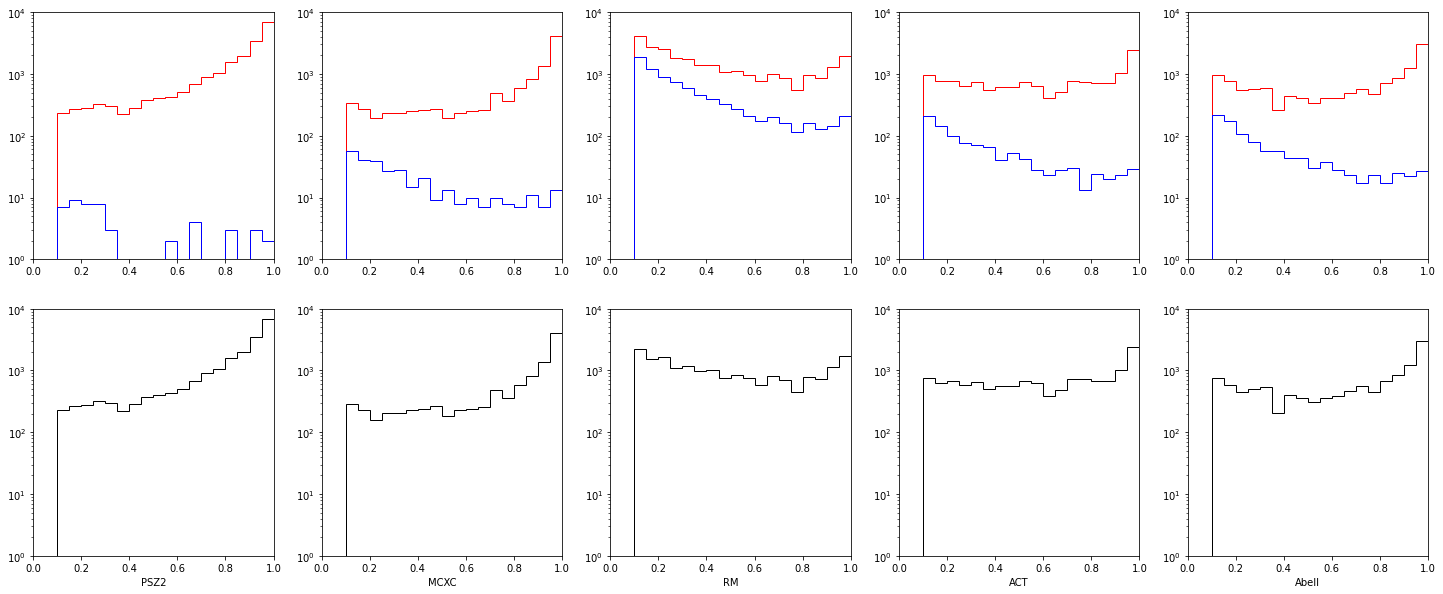
\includegraphics[width=\linewidth]{hist_old}
\caption{Распределение всех найденных объектов и ошибочно найденных объектов, а также разница между 
ними (старая версия алгоритма)}
\label{Fig:Hist_old}
\end{figure}
\begin{figure}[h]
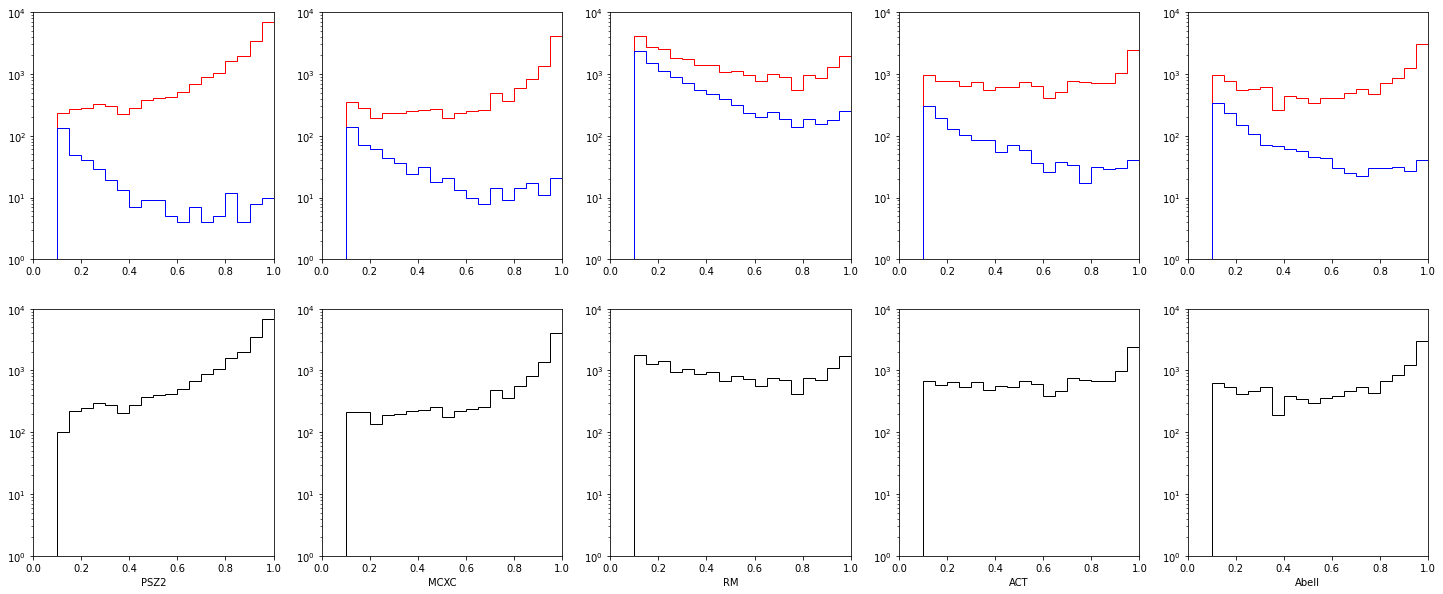
\includegraphics[width=\linewidth]{hist_new}
\caption{Распределение всех найденных объектов и ошибочно найденных объектов, а также разница между 
ними (новая версия алгоритма)}
\label{Fig:Hist_new}
\end{figure}

\begin{figure}[h]
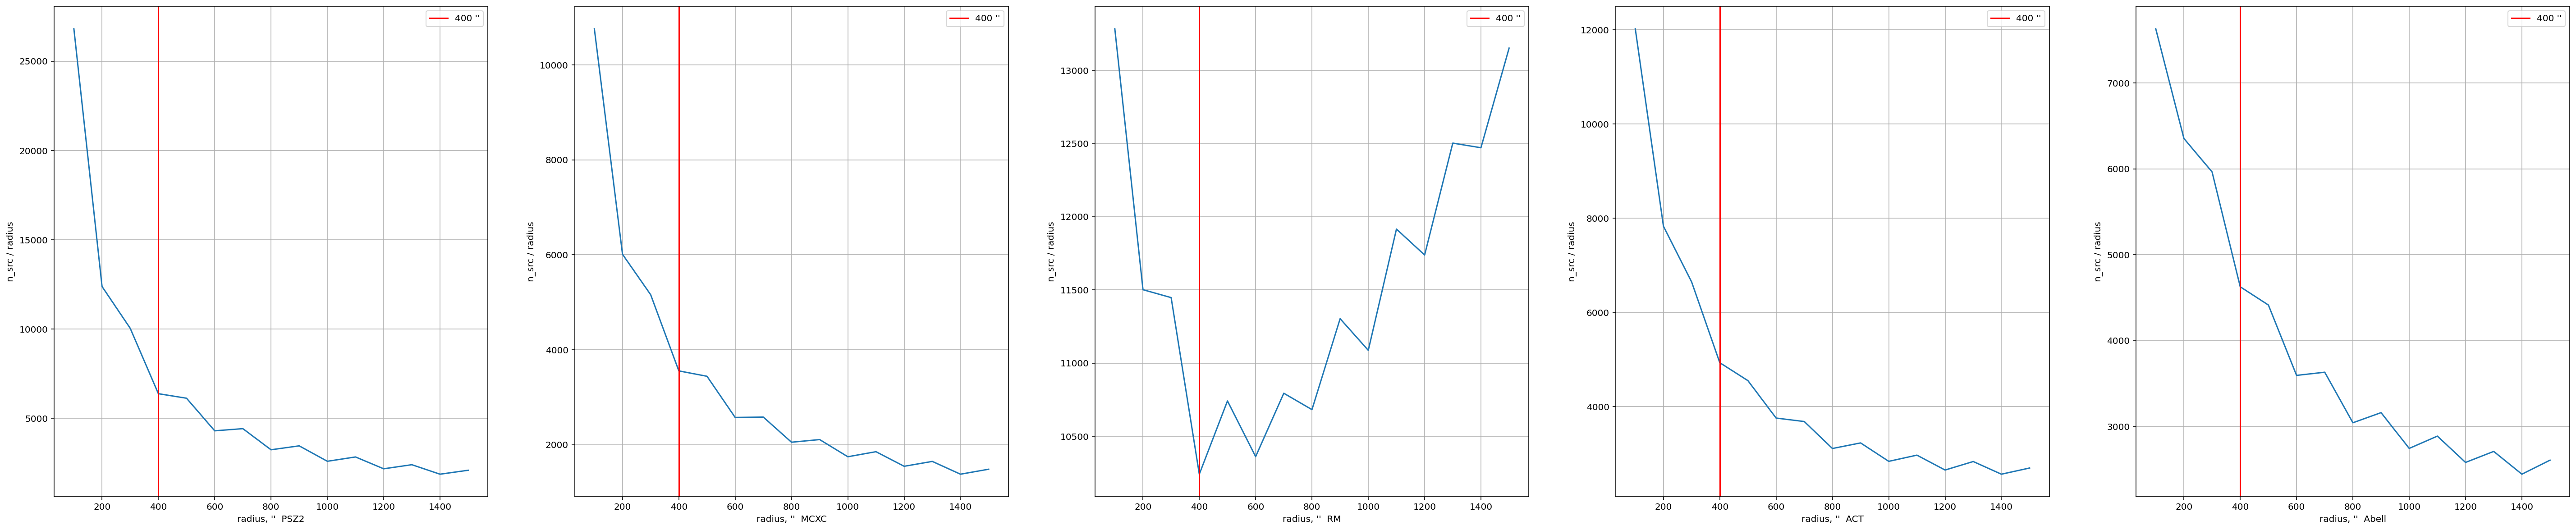
\includegraphics[width=\linewidth]{rad}
\caption{Количество найденных объектов в зависимости от радиуса (дифференцированный график)}
\label{Fig:rad}
\end{figure}
Отчет согласован с научным руководителем.\\
Общее количество строк кода за эту неделю: 56\\
\href{https://github.com/rt2122/data-segmentation-2}{Репозиторий}\\ 
\end{document}
